%%
%% This is file `elsarticle-template-num.tex',
%% generated with the docstrip utility.
%%
%% The original source files were:
%%
%% elsarticle.dtx  (with options: `numtemplate')
%% 
%% Copyright 2007, 2008 Elsevier Ltd.
%% 
%% This file is part of the 'Elsarticle Bundle'.
%% -------------------------------------------
%% 
%% It may be distributed under the conditions of the LaTeX Project Public
%% License, either version 1.2 of this license or (at your option) any
%% later version.  The latest version of this license is in
%%    http://www.latex-project.org/lppl.txt
%% and version 1.2 or later is part of all distributions of LaTeX
%% version 1999/12/01 or later.
%% 
%% The list of all files belonging to the 'Elsarticle Bundle' is
%% given in the file `manifest.txt'.
%% 

%% Template article for Elsevier's document class `elsarticle'
%% with numbered style bibliographic references
%% SP 2008/03/01

%\documentclass[preprint,12pt]{elsarticle}
\documentclass[preprint,10pt]{elsarticle}
%\documentclass[final,3p,times]{elsarticle} 

%% Use the option review to obtain double line spacing
%% \documentclass[authoryear,preprint,review,12pt]{elsarticle}

%% Use the options 1p,twocolumn; 3p; 3p,twocolumn; 5p; or 5p,twocolumn
%% for a journal layout:
%% \documentclass[final,1p,times]{elsarticle}
%% \documentclass[final,1p,times,twocolumn]{elsarticle}
%% \documentclass[final,3p,times]{elsarticle}
%% \documentclass[final,3p,times,twocolumn]{elsarticle}
%% \documentclass[final,5p,times]{elsarticle}
%% \documentclass[final,5p,times,twocolumn]{elsarticle}

%% if you use PostScript figures in your article
%% use the graphics package for simple commands
\usepackage{subfigure}

\usepackage{color}
%% or use the graphicx package for more complicated commands
\usepackage{graphicx}
%% or use the epsfig package if you prefer to use the old commands
%% \usepackage{epsfig}

%% The amssymb package provides various useful mathematical symbols 
%% The amsthm package provides extended theorem environments
\usepackage{amssymb}
\usepackage{amsmath}
% more math
\usepackage{amsfonts}
\usepackage{amstext}
\usepackage{amsbsy}
\usepackage{mathbbol} 

%% The lineno packages adds line numbers. Start line numbering with
%% \begin{linenumbers}, end it with \end{linenumbers}. Or switch it on
%% for the whole article with \linenumbers.
\usepackage{lineno}

\journal{Journal of Comp. Phys.}
%%%%%%%%%%%%%%%%%%%%%%%%%%%%%%%%%%%%%%%%%%%%%%%%%%%%%%%%%%%%%%%%%%%%
% operators
\renewcommand{\div}{\vec{\nabla}\! \cdot \!}
\newcommand{\grad}{\vec{\nabla}}
% latex shortcuts
\newcommand{\bea}{\begin{eqnarray}}
\newcommand{\eea}{\end{eqnarray}}
\newcommand{\be}{\begin{equation}}
\newcommand{\ee}{\end{equation}}
\newcommand{\bal}{\begin{align}}
\newcommand{\eali}{\end{align}}
\newcommand{\bi}{\begin{itemize}}
\newcommand{\ei}{\end{itemize}}
\newcommand{\ben}{\begin{enumerate}}
\newcommand{\een}{\end{enumerate}}
% DGFEM commands
\newcommand{\jmp}[1]{[\![#1]\!]}                     % jump
\newcommand{\mvl}[1]{\{\!\!\{#1\}\!\!\}}             % mean value
\newcommand{\keff}{\ensuremath{k_{\textit{eff}}}\xspace}
% shortcut for domain notation
\newcommand{\D}{\mathcal{D}}
% vector shortcuts
\newcommand{\vo}{\vec{\Omega}}
\newcommand{\vr}{\vec{r}}
\newcommand{\vn}{\vec{n}}
\newcommand{\vnk}{\vec{\mathbf{n}}}
\newcommand{\vj}{\vec{J}}

\newcommand{\EI}{\mathcal{E}_h^i}
\newcommand{\ED}{\mathcal{E}_h^{\partial \D^d}}
\newcommand{\EN}{\mathcal{E}_h^{\partial \D^n}}
\newcommand{\ER}{\mathcal{E}_h^{\partial \D^r}}
\newcommand{\reg}{\textit{reg}}

% extra space
\newcommand{\qq}{\quad\quad}
% common reference commands
\newcommand{\eqt}[1]{Eq.~(\ref{#1})}                     % equation
\newcommand{\fig}[1]{Fig.~\ref{#1}}                      % figure
\newcommand{\tbl}[1]{Table~\ref{#1}}                     % table
\newcommand{\sct}[1]{Section~\ref{#1}}                   % section

\newcommand\br{\mathbf{r}}
%\newcommand{\tf}{\varphi}
\newcommand{\tf}{b}

\newcommand{\tcr}[1]{\textcolor{red}{#1}}
\newcommand{\mt}[1]{\marginpar{ {\tiny #1}}}
%%%%%%%%%%%%%%%%%%%%%%%%%%%%%%%%%%%%%%%%%%%%%%%%%%%%%%%%%%%%%%%%%%%%%
%
%   BEGIN DOCUMENT
%
%%%%%%%%%%%%%%%%%%%%%%%%%%%%%%%%%%%%%%%%%%%%%%%%%%%%%%%%%%%%%%%%%%%%%
\begin{document}

 

%%%%%%%%%%%%%%%%%%%%%%%%%%%%%%%%%%%%%%%%%%%%%%%%%%%%%%%%%%%%%%%%%%%%
\begin{frontmatter}

%% Title, authors and addresses

%% use the tnoteref command within \title for footnotes;
%% use the tnotetext command for theassociated footnote;
%% use the fnref command within \author or \address for footnotes;
%% use the fntext command for theassociated footnote;
%% use the corref command within \author for corresponding author footnotes;
%% use the cortext command for theassociated footnote;
%% use the ead command for the email address,
%% and the form \ead[url] for the home page:
%\title{Title\tnoteref{label1}}
%% \tnotetext[label1]{}
%% \author{Name\corref{cor1}\fnref{label2}}
%% \ead{email address}
%% \ead[url]{home page}
%% \fntext[label2]{}
%% \cortext[cor1]{}
%% \address{Address\fnref{label3}}
%% \fntext[label3]{}

%-------------------------
%-------------------------
%\title{Discontinuous Finite Element Solution for Diffusion Equations on Arbitrary Polygonal Meshes}
\title{Discontinuous Finite Element Solution of the Diffusion Equation on Arbitrary Polygonal Meshes}
%-------------------------
%-------------------------

%% use optional labels to link authors explicitly to addresses:
%% \author[label1,label2]{}
%% \address[label1]{}
%% \address[label2]{}

%-------------------------
\author{Jean C. Ragusa\fnref{label1}\corref{cor1}}
\ead{jean.ragusa@tamu.edu}

% \cortext[cor1]{Corresponding author}
%-------------------------

%-------------------------
\begin{abstract}

aaaa

\end{abstract}
%-------------------------

%-------------------------
\begin{keyword}
  Radiation Diffusion \sep
	Arbitrary Polygonal Grids \sep
  Discontinuous Finite Element \sep
  Piecewise Linear Discontinuous \sep
  Adaptive Mesh Refinement\, .
\end{keyword}
%-------------------------

\end{frontmatter}

%%%%%%%%%%%%%%%%%%%%%%%%%%%%%%%%%%%%%%%%%%%%%%%%%%%%%%%%%%%%%%%%%%%%

\linenumbers

%%%%%%%%%%%%%%%%%%%%%%%%%%%%%%%%%%%%%%%%%%%%%%%%%%%%%%%%%%%%%%%%%%%%%%%%%%%%%%%%%%%%%%%%%%%%%%%%%%%%
%%%%%%%%%%%%%%%%%%%%%%%%%%%%%%%%%%%%%%%%%%%%%%%%%%%%%%%%%%%%%%%%%%%%%%%%%%%%%%%%%%%%%%%%%%%%%%%%%%%%
\section{Introduction} \label{sec:intro}
%%%%%%%%%%%%%%%%%%%%%%%%%%%%%%%%%%%%%%%%%%%%%%%%%%%%%%%%%%%%%%%%%%%%%%%%%%%%%%%%%%%%%%%%%%%%%%%%%%%%
%%%%%%%%%%%%%%%%%%%%%%%%%%%%%%%%%%%%%%%%%%%%%%%%%%%%%%%%%%%%%%%%%%%%%%%%%%%%%%%%%%%%%%%%%%%%%%%%%%%%

\tcr{Make sure the following is expressed somewhere:\\
In this
research, we focus on using PWLD to discretize the diffusion equation. The
PWLD discretization employs discontinuous finite elements and has been used to
discretize the transport equation. Using it to discretize the diffusion
equation is an important step in order to create a Diffusion Synthetic
Acceleration scheme \cite{Adams2002,Wang2010}.
}
\bigskip

This paper deals with a discontinuous finite element spatial discretization of the radiation 
diffusion equation on arbitrary polygonal grids, with and without adaptive mesh refinement. 
Radiation diffusion is an asymptotic limit of the radiation transport equation and can be 
written in the following form:
\begin{equation} \label{eq:radiation_diffusion}
- \div  D(\vr) \grad E(\vr) + \sigma_a(\vr) E(\vr) = Q(\vr) ,
\end{equation}
where $E$ is the radiation energy intensity, $D$ is a diffusion coefficient, $\sigma_a$ is 
an opacity coefficient, and $Q$ is the source.

Several spatial discretizations have been proposed to solve \eqt{eq:radiation_diffusion} on
arbitrary polygons (2D) and polyhedra (3D) \cite{Wachspress,Kuznetsov2004,Palmer2005,Brezzi2005,
LipnikovShashkovSvyatskiy2006,BaileyAdams2008}. We review them below.
%
Wachspress \cite{Wachspress} developed a family of rational polynomial functions that can be employed
as basis functions in a finite element method on polygonal/polyhedral grids. This yields
symmetric positive-definite (SPD) matrices but (i) the finite element integrals must be carried out 
numerically and (ii) the Jacobian of the transformation becomes zero on degenerate cells 
(such as the ones shown on \fig{fig:amr_schematics}) and on non-convex cells. 
%
%Morel et al. \cite{MorelDendyHallWhite1992} introduced a cell-centered finite volume scheme 
%for arbitrary quadrilateral meshes. Their scheme was second-order accurate and yielded back a 
%standard five-point stencil on orthogonal grids, but the diffusion operator was asymmetric 
%and cell-edge unknowns were added in addition to cell-center unknowns.
%%
Palmer \cite{Palmer2005,PalmerLLNL} proposed a node-based finite volume method 
that enforces particle balance over the control volume associated with a given grid vertex.
This control volume defines a dual cell constructed as 
the union of all corners surrounding the specified vertex $v$. In 2D, a corner 
is a quadrilateral with the following vertices: vertex $p$, the cell center, and the midpoint
of the edges that contain vertex $p$. On a triangular grid, Palmer's scheme is equivalent 
to employing linear continuous finite elements with ``mass-matrix lumping''. This method is 
second-order accurate but its discretization of the diffusion equation produces an 
asymmetric (i.e., not SPD) matrix, in general.
%
Mimetic finite difference methods create discrete analog of vector and tensor
calculus in order to accurately approximate the original differential operators;
see, e.g., \cite{HymanMorelShashkovSteinberg2002}.
Mimetic methods preserve important properties of the differential operators such 
as symmetry, positivity, monotonicity, asymptotic limits, and identities pertaining 
to tensor and vector calculus. Mimetic methods can also be viewed as mixed hybrid 
finite element formulations with specific spatial quadratures.  
In addition to quadrilateral and hexahedral meshes (see, e.g., 
\cite{MorelRobertsShashkov1998,MorelHallShashkov2001}, mimetic finite difference 
methods have recently been applied to the diffusion equation on arbitrary polygonal 
grids \cite{Kuznetsov2004,Brezzi2005,LipnikovShashkovSvyatskiy2006,LipnikovShashkov2010}.
%conformal quadrilateral \cite{HymanShashkovSteinberg1997, ShashkovSteinberg1996,MorelRobertsShashkov1998} 
%and hexahedral \cite{MorelHallShashkov2001} grids, locally refined grids \cite{LipnikovMorelShashkov2004}, and
%arbitrary polygonal grids \cote{Kuznetsov2004,Brezzi2005,LipnikovShashkovSvyatskiy2006,LipnikovShashkov2010}.
%
Bailey et al. \cite{BaileyAdams2008} recently employed piecewise linear basis
functions to solve a diffusion equation using a Galerkin finite element technique on 
arbitrary polygonal and polyhedral grids. Their goal was to devise a {\em continuous} finite 
element discretization that does not necessitate numerical integration, yields an SPD matrix, 
is second-order accurate, and handles arbitrary polygonal/polyhedral grids (including 
grids with degenerate cells). The approach they followed is a standard Galerkin weak 
formulation for continuous finite elements, with piecewise linear basis functions 
defined on subcells (which they called ``sides'') of arbitrary polygons/polyhedrons.

In this paper, we are interested in solving a diffusion equation on arbitrary polygonal
grids using a {\em discontinuous} finite element discretization. We employ the
Symmetric Interior Penalty (SIP) technique \cite{IPRefs}, developed for the discretization
of elliptic equations using discontinuous Galerkin techniques. For basis functions,
we use the piecewise linear functions of \cite{BaileyAdams2008}.
The motivations are three-fold: 
\begin{enumerate}
\item we wish to assess the performance of the discontinuous finite elements for 
	the discretization of the diffusion equation on polygonal meshes;
\item a diffusion equation often serves as a synthetic accelerator or 
	preconditioner for iterative solution techniques applied to particle transport
	\cite{AdamsLarsen2002}. A discontinuous finite element technique is often employ
	in the discretization of the transport equation for unstructured and 
	polygonal/polyhedral grids \cite{MorelWarsaWareing,PWLD,CFEM-PWDL-Warsa,WangRagusa}.
  Employing the same    
\item 
\end{enumerate}
The motivations for our work / In this work, we wish to assess ... In addition,
a diffusion equation often serves as a synthetic accelerator or as a
preconditioner \cite{AdamsLarsen2002} for iterative solution techniques of the 
radiation transport equation.
% , where a discontinuous finite element technique is often preferred
% in the discretization of the transport equation for unstructured and 
% polygonal/polyhedral grids \cite{MorelWarsaWareing,PWLD,CFEM-PWDL-Warsa,WangRagusa}.

The remainder of the paper is as follows. In \sct{sec:poly}, we discuss
the use of polygonal meshes, define the piecewise linear discontinuous 
basis functions for arbitrary polygons, and discuss how polygonal grids
can be utilized in handling local mesh refinement (as in adaptive mesh refinement 
approaches). The Symmetric Interior Penalty technique is reviewed in \sct{sec:ip}.
%The resulting linear system will be solved using an Algebraic Multi-Grid (AMG) approach.
Mesh adaptivity utilizing piecewise linear basis function is presented in 
\sct{sec:amr}. Results are provided in \sct{sec:results}; all of the test cases presented
are borrowed from the literature on (1) finite differences applied to the
diffusion equation on non FINISH 

%%%%%%%%%%%%%%%%%%%%%%%%%%%%%%%%%%%%%%%%%%%%%%%%%%%%%%%%%%%%%%%%%%%%%%%%%%%%%%%%%%%%%%%%%%%%%%%%%%%%
%%%%%%%%%%%%%%%%%%%%%%%%%%%%%%%%%%%%%%%%%%%%%%%%%%%%%%%%%%%%%%%%%%%%%%%%%%%%%%%%%%%%%%%%%%%%%%%%%%%%
\section{Polygonal Grids and Piecewise Linear Basis Functions} \label{sec:poly}
%%%%%%%%%%%%%%%%%%%%%%%%%%%%%%%%%%%%%%%%%%%%%%%%%%%%%%%%%%%%%%%%%%%%%%%%%%%%%%%%%%%%%%%%%%%%%%%%%%%%
%%%%%%%%%%%%%%%%%%%%%%%%%%%%%%%%%%%%%%%%%%%%%%%%%%%%%%%%%%%%%%%%%%%%%%%%%%%%%%%%%%%%%%%%%%%%%%%%%%%%
%-----------------------------------------------------------
\subsection{Polygonal Meshes and their Application to Adaptive Mesh Refinement}
%-----------------------------------------------------------

Polygonal cells are an alternative to standard (triangles/quads) mesh partitioning.
Mesh generation using polygons (polyhedra in 3D) is an active area of research.
Some meshing tools, such as MSTK \cite{mstk} and the Computational Geometry Algorithms 
Library \cite{cgal}, may be employed to generate/process polygonal meshes.  
Several CFD codes (Fluent, StarCCM, OpenFoam) also offer polygonal meshing and solver capabilities. 

The rationale for polygonal/polyhedral cells is as follows.
While quadrilaterals (hexahedra in 3D) can be seen as the standard cell shapes for logically 
structured meshes, they may be difficult to employ in complex geometries. For unstructured meshes,
triangles (tetrahedra in 3D) are the typical building blocks and are employed in 
numerous automated meshing algorithms, but are not well-suited for boundary layers, 
for instance, and may require higher cell counts than quad/hex meshes for a similar
resolution.  The following features of polygonal cells are noteworthy:
\begin{itemize}
  \item They can provide a better partition of the domain, minimizing the boundary/interior ratio;
  \item The number of unknowns for an equivalent accuracy/resolution can be reduced (similar to the advantages of 
	hex meshes over tet meshes);
	\item The notion of transition elements is included by default in arbitrary grids composed of
	polygons/polyhedra. Therefore, such a grid can easily be split by cut planes, for 
	instance. 
  \item The notion of ``hanging nodes'' for locally refined/adapted meshed is no longer needed.
	For example, \fig{fig:amr1} shows two quadrilateral elements before local refinement; on
	\fig{fig:amr2}, one of the two cells has been refined. The un-refined cell is now viewed as a
	pentagon.
\end{itemize}

\begin{figure}[!hbtp]
\centering
%\vspace{40mm}
%\hspace{-55mm}
\subfigure[before local refinement]{
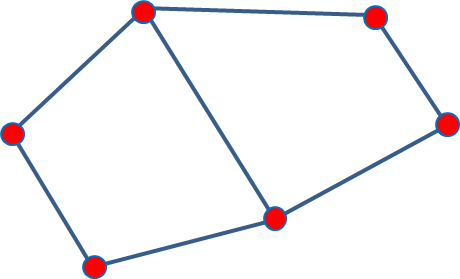
\includegraphics[scale=0.55]{amr1.png}
\label{fig:amr1}
}
%\hspace{45mm}
\subfigure[after local refinement]{
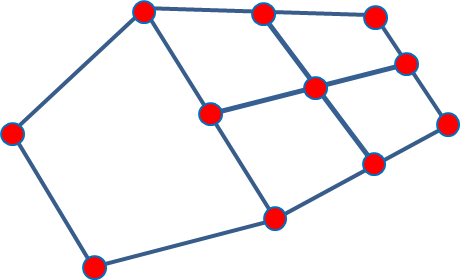
\includegraphics[scale=0.55]{amr2.png}
\label{fig:amr2}
}
\caption{Local mesh refinement leads to pentagonal cell}
\label{fig:amr}
\end{figure}


%-----------------------------------------------------------
\subsection{Piecewise Linear Basis Functions on Arbitrary Polygons}
%-----------------------------------------------------------

Consider a polygonal cell with $N_V$ vertices, $(x_i,y_i)$. The polygon needs not 
to be convex. In order to describe the piecewise linear basis functions
for such a cell, we introduce a cell ``center'', denoted hereafter 
by $c=(x_c,y_c)$, with $x_c =\sum_{i=1}^{N_V} \alpha_{i} x_i$
and  $y_c = \sum_{i=1}^{N_V} \alpha_{i} y_i$. We require that
$\sum_{i=1}^{N_V} \alpha_{i} = 1$. Thus, point $c$ can be interpreted as 
a weighted average of the polygon's vertices. Often, one chooses 
$\alpha_i = 1 / N_V$ but one may also define point $c$ as the centroid of the
polygon under consideration.
With the introduction of the cell center, the polygon can be viewed as
$N_V$ triangular subcells (or ``sides'' if using the terminolgy of \cite{bailey}), 
each of these triangles being composed of two
successive vertices and the cell center.
The $N_V$ piecewise linear basis functions are then given by:
%
\begin{equation}
  b_j(\br) = t_j(\br) + \alpha_{j} t_c(\br) , \qquad j=1,\ldots,N_V ,
\end{equation}
%
where $t_j(\br)$ is the standard linear function defined on the two adjacent
triangular subcells formed by (1) vertex $j$, vertex $j-1$ and the cell center $c$,
and (2) vertex $j$, vertex $j+1$ and the cell center $c$.
$t_j$ is equal to one at the $j^{th}$ vertex and to zero at all other vertices of the polygon,
as well as at the cell center.
$t_c(\br)$ is the ``tent'' function associated with the cell center and is equal to one 
at the cell center and to zero at all of the polygon vertices.
%
We stress that this choice of basis functions is not equivalent to employing a standard 
continuous finite element representation within a polygon that would divide such a polygon 
into $N_V$ triangular subcells. Indeed, in the case of a standard continuous finite 
element representation, the number of basis functions would be $N_V+1$ 
(for the $N_V$ vertices and the cell center). In the
piecewise linear representation, the unknowns are only located at the cell 
vertices and the cell center point is only used to define the basis functions.
For example, \fig{fig:pentagons} presents two simple examples of polygonal cells: a 
pentagon and a degenerated pentagon, the later is typically obtained
during local mesh adaptation (see also \fig{fig:amr2}).
The isolines of the piecewise linear basis functions for vertex $D$ and
$E$ are graphed in \fig{fig:pwl_pentagon} for the regular pentagon
and in \fig{fig:pwl_degen_pentagon} for the degenerate pentagon.
%
\begin{figure}[!hbtp]
\centering
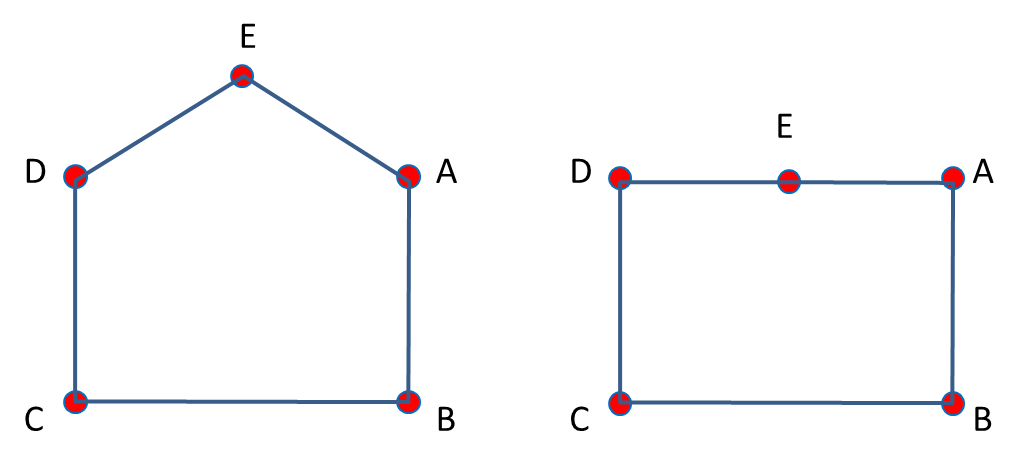
\includegraphics[scale=0.77]{pentagons.png}
\label{fig:pentagons}
\caption{Non-degenerate (left) and degenerate (right) pentagonal cells}
\end{figure}
%
%
\begin{figure}[!hbtp]
\centering
\subfigure[Basis function for Point D]{
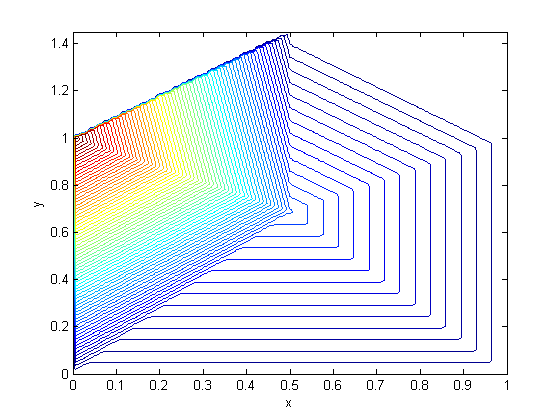
\includegraphics[scale=0.33]{PWL_D.png}
\label{fig:pwl_pentagonD}
}
\subfigure[Basis function for Point E]{
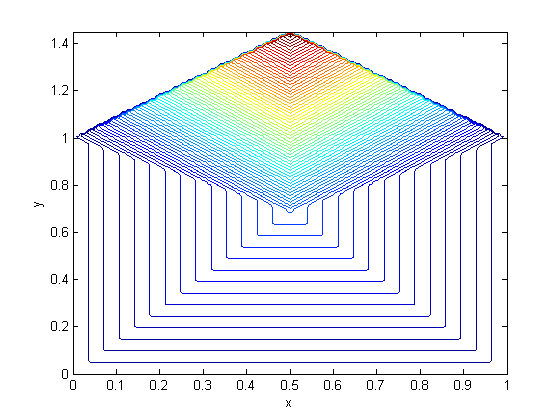
\includegraphics[scale=0.33]{PWL_E.png}
\label{fig:pwl_pentagonE}
}
\caption{Isolines of PWL basis functions for a non-degenerate pentagon}
\label{fig:pwl_pentagon}
\end{figure}
%
\begin{figure}[!hbtp]
\centering
\subfigure[Basis function for Point D]{
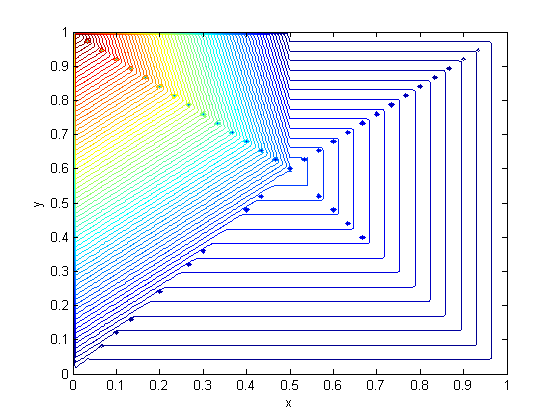
\includegraphics[scale=0.33]{PWL_D_flat.png}
\label{fig:pwl_degen_pentagonD}
}
\subfigure[Basis function for Point E]{
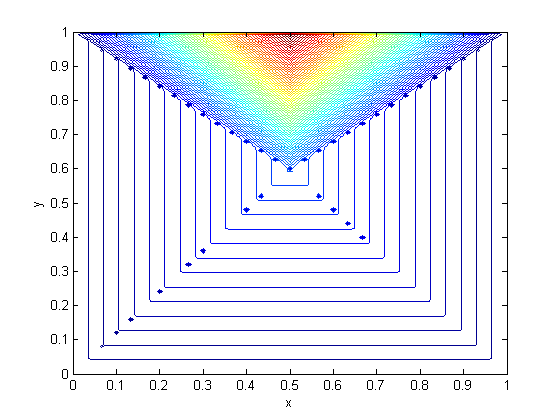
\includegraphics[scale=0.33]{PWL_E_flat.png}
\label{fig:pwl_degen_pentagonE}
}
\caption{Isolines of PWL basis functions for a degenerate pentagon}
\label{fig:pwl_degen_pentagon}
\end{figure}



%%%%%%%%%%%%%%%%%%%%%%%%%%%%%%%%%%%%%%%%%%%%%%%%%%%%%%%%%%%%%%%%%%%%%%%%%%%%%%%%%%%%%%%%%%%%%%%%%%%%
%%%%%%%%%%%%%%%%%%%%%%%%%%%%%%%%%%%%%%%%%%%%%%%%%%%%%%%%%%%%%%%%%%%%%%%%%%%%%%%%%%%%%%%%%%%%%%%%%%%%
\section{Discontinuous Finite Element Formulation} \label{sec:ip}
%%%%%%%%%%%%%%%%%%%%%%%%%%%%%%%%%%%%%%%%%%%%%%%%%%%%%%%%%%%%%%%%%%%%%%%%%%%%%%%%%%%%%%%%%%%%%%%%%%%%
%%%%%%%%%%%%%%%%%%%%%%%%%%%%%%%%%%%%%%%%%%%%%%%%%%%%%%%%%%%%%%%%%%%%%%%%%%%%%%%%%%%%%%%%%%%%%%%%%%%%

In this Section, we present the discontinuous Galerkin finite element technique employed to
discretize the radiation diffusion equation on arbitrary polygonal grids. Many variants of such discretization
methods exist for diffusion problems (depending on the choice of stabilization terms, whether 
the diffusion equation is expressed in its mixed form, \ldots). We refer the Readers to the review
papers \cite{unification,brezzi etc} for additional details. Here, we employ the Symmetric
Interior Penalty (SIP) method which we have found to be robust in our test cases and relatively simple 
to implement.
%Even though discontinuous Galerkin methods are commonly used in the particle and radiation transport communities, 
The general idea of interior penalty methods can be traced back to \cite{lions1968}, where the Dirichlet
boundary conditions to the model diffusion problem $\{-\div \grad E = Q$ in domain $\D$, $E=E^d$ on 
the boundary $\partial \D\}$ have been enforced via a penalty method, thereby modifying the 
boundary condition to read $E+\frac{1}{\mu}\partial_n E = E^d$ with $\mu\gg 1$. Later, 
Nitsche \cite{nitsche1971} proposed a consistent formulation for the enforcement of the 
Dirichlet boundary condition with a penalty term, leading to the weak formulation:
\begin{equation}
\label{eq:penalty_nitsche_bd_only}
\int_{\D} \grad E \cdot \grad \tf
- \int_{\partial\D} \partial_n E \tf  
- \int_{\partial\D} \partial_n \tf E 
+ \int_{\partial\D} \mu(E-E^d) \tf 
=
\int_{\D} Q \tf 
- \int_{\partial\D} E^d \partial_n \tf ,
\end{equation}
with $\tf$ a finite element basis function and $\mu=\alpha/h$, where $h$ denotes 
the mesh size and $\alpha>1$ is a constant.
%
Nitsche's idea, extended to all cell edges (not only cells with edges on the boundary), leads
to the family of interior penalty methods for discontinuous finite elements. The SIP form,
which we have chosen here because it is one of the simplest forms and leads to symmetric 
positive definite matrices, is discussed next. 

First, we recall \eqt{eq:radiation_diffusion} and specify 
Dirichlet, Neumann, and Robin boundary condition types on various portions the the domain's
boundary:
\begin{equation}
  -\div D(\vr) \grad E(\vr) + \sigma_a(\vr) E(\vr) = Q(\vr)\ \textrm{ for } \vr \in \D,
\end{equation}
with Dirichlet boundary conditions
\begin{equation}
  E(\vr)  = E_0(\vr)\ \textrm{ for } \vr \in  \partial \D^d \, ,
\end{equation}
Neumann boundary conditions
\begin{equation}
  -D \partial_n E(\vr) = F_0(\vr) \ \textrm{ for } \vr \in \partial \D^n,
\end{equation}
and Robin boundary conditions
\begin{equation}
  \frac{1}{4}E(\vr) + \frac{1}{2} D(\vr) \partial_n E(\vr) = F^{inc}(\vr) \ \textrm{ for } \vr \in  \partial \D^r \, .
\end{equation}
%
where $E$ is the unknown radiation scalar intensity. The boundary of the domain is split as
$\partial \D = \partial \D^d \cup \partial \D^n \cup \partial \D^r$,  where the superscripts
denote Dirichlet, Neumann, and Robin types, respectively. $E_0$, $F_0$, and $F^{inc}$ are specified
quantities. $\partial_n \boxdot$ denotes $ \grad \boxdot \cdot \vn$ with $vn$ the outward unit normal vector.


% Obviously, the domain boundary is the  $\partial \D = \mathcal{E}_h^{\partial\D,D}\cup \mathcal{E}_h^{\partial\D,N} \cup \mathcal{E}_h^{\partial\D,R}$.
%-----------------------------------------------------------
\subsection{The Symmetric Interior Penalty (SIP) Method}
%-----------------------------------------------------------

In this paragraph, we describe the SIP discretization \cite{Kanschat2007} of the 
radiation diffusion equation using discontinuous finite elements. 
We introduce a partition
of the domain, $\bigcup\nolimits_{K\in \mathbb{T}_{h}}K=\D$, and also assume
that the boundary of the domain, $\partial \D$, consists of straight edges only. The 
set of interior and boundary edges is denoted by $\EI$ and $\mathcal{E}_h^{\partial\D}$,
respectively; the set of boundary edges is further split into the three different boundary 
condition types, i.e., $\mathcal{E}_h^{\partial\D} = \ED \cup \EN \cup \ER$. 
Then, the SIP formulation is given by
\begin{multline}
\label{eq:SIP_1}
\int_{\mathbb{T}_{h}} \Big( D \grad E \cdot \grad \tf + \sigma_a E \tf \Big)
+ \int_{\EI} \Big( \mvl{D\partial_n E} \jmp{\tf}  + \mvl{D\partial_n \tf} \jmp{E} + \kappa\jmp{E}\jmp{\tf} \Big)
\\
+ \int_{\ED} \Big( \kappa E \tf -D\tf \partial_n E  -D E \partial_n \tf \Big)
+ \frac{1}{2} \int_{\ER}  E \tf  
\\
=
\int_{\mathbb{T}_{h}} Q \tf 
+ \int_{\ED} E_0 \Big( \kappa \tf  -D \partial_n \tf  \Big)
- \int_{\EN} F_0 \tf  
+ \int_{\ER} 2 F^{inc} \tf  \, ,
\end{multline}
where we recall that $\tf$ is a generic test function. 
In \eqt{eq:SIP_1}, the last term on the left-hand side and the last two terms on the right-hand side 
are naturally obtained by applying the Neumman and Robin boundary conditions. The terms pertaining 
to the Dirichlet boundary conditions are identical to the ones of Nitsche's penalty method. 
Finally, the interior edge terms are the standard terms due to the extension of Nitsche's method to 
the interior edges (see also \cite{qqq}). To generate the linear system associated with \eqt{eq:SIP_1}, 
we have opted to use two loops: one over the elements to compute the volume integrals,
\begin{equation}
\int_{\mathbb{T}_{h}} \longrightarrow \sum_{K \in \mathbb{T}_{h}} \int_{K} \, ,
\end{equation}
and one of the edge sets to compute the edge integrals
\begin{equation}
\int_{\mathcal{E}_h} \longrightarrow \sum_{e \in \mathcal{E}_h} \int_{e} \, .
\end{equation}
We have also chosen to arbitrarily assign a unit normal vector, $\vn$, to each interior edge (for the boundary edges,
$\vn$ is always to outward point unit normal vector). With this choice, the definition of the mean value and the jump of a quantity $u$ on any given interior edge are given by
\begin{equation} \label{eq:mean}
\mvl{u} = \frac{u^+ + u^-}{2}
\end{equation}
and
\begin{equation} \label{eq:jump}
\jmp{u} = u^+ - u^- \, ,
\end{equation}
respectively.  The values taken by the quantity $u$ while approaching the edge from either one of its sides are defined as follows:
\begin{equation} \label{eq:upm}
u^\pm = \lim_{s\to 0^\pm} u(\vr + s \vn) \, ,
\end{equation}
for any point $\vr$ on that edge (that is, $u^+$ is the trace of $u$ along that edge taken from the cell pointed by $\vn$).
%
The penalty coefficient, $\kappa$, is edge-dependent and is given by
\begin{equation} \label{eq:kappa}
  \kappa_e = \left\{
    \begin{array}{ll}
      \frac{C}{2} \left( \frac{D^+}{h_\bot^+} + \frac{D^-}{h_\bot^-} \right) & \textrm{ for interior edges, i.e., } e \in \EI,\\
      2C \frac{D^-}{h_\bot^-}  & \textrm{ for boundary edges, i.e., } e \in \partial \mathcal{E}_h^{\partial\D}
    \end{array}
    \right. \, ,
\end{equation}
where $C$ is a constant, $h_{\bot}$ is the length of the cell in the direction 
orthogonal to edge $e$. 
%In the mathematical literature, the jumps terms, $\kappa\jmp{E}\jmp{\tf}$,
%are also identified as a stabilization technique for which the constant $\kappa$ needs to be large enough. 
For quadrilateral meshes with linear basis functions, researchers typically utilize $C \ge 4$ 
(through the formula $C=c(p+1)^2$, with $c\ge 1$ and $p$ the polynomial order). Here, we use $C=4$
unless otherwise noted. For boundary edges, 
Kanschat \cite{Kanschat2007} noted that doubling the value of $C$ (on quadrilateral meshes) was 
beneficial; we have followed their recommendations. In \eqt{eq:kappa}, the $\pm$ superscripts 
represent again values taken from either side of an edge. For triangular cells, $h_\bot$ is exactly 
given by $h_{\bot}=\frac{2A}{L_e}$ where $A$ is the triangle area and $L_e$ is the length of edge $e$. 
However, there are no formulae to compute $h_{\bot}$ for arbitrary polygons. In \cite{BT-PhD}, 
polygonal cells were assumed to be regular polygonal cells, in which case $h_{\bot}^\reg$ is given
by twice the inradius for regular even-sided polygons and by the inradius plus the 
circumradius for odd-sided polygons. The inradius and the circumradius are computed 
using the area and perimeter of the actual polygonal cell. 
%For highly skewed meshes, 
%One possible disadvantage of assuming 
%that the cells are regular polygons is that the same value of $h_{\bot}$ is used for all edges.
%For highly skewed polygons, that value can be either too small or too large. Too small a value for 
%$h_{\bot}$ increases the penalty coefficient $\kappa$, hence augments the value of stabilization 
%terms even further, which is not an issue. However, when the assumption of a regular polygon leads to
%$h_{\bot}$ values that are too large, $\kappa$ may not be large enough.




%%%%%%%%%%%%%%%%%%%%%%%%%%%%%%%%%%%%%%%%%%%%%%%%%%%%%%%%%%%%%%%%%%%%%%%%%%%%%%%%%%%%%%%%%%%%%%%%%%%%
%%%%%%%%%%%%%%%%%%%%%%%%%%%%%%%%%%%%%%%%%%%%%%%%%%%%%%%%%%%%%%%%%%%%%%%%%%%%%%%%%%%%%%%%%%%%%%%%%%%%
\section{Adaptive Mesh Refinement Using PWLD Basis Functions} \label{sec:amr}
%%%%%%%%%%%%%%%%%%%%%%%%%%%%%%%%%%%%%%%%%%%%%%%%%%%%%%%%%%%%%%%%%%%%%%%%%%%%%%%%%%%%%%%%%%%%%%%%%%%%
%%%%%%%%%%%%%%%%%%%%%%%%%%%%%%%%%%%%%%%%%%%%%%%%%%%%%%%%%%%%%%%%%%%%%%%%%%%%%%%%%%%%%%%%%%%%%%%%%%%%

Solutions with strong and rapid spatial variations can be accurately captured using mesh adaptivity
\cite{amr_stuff}. Adaptive Mesh Refinement (AMR) techniques require local error estimates to determine
which cells to refine. When using discontinuous finite elements, the numerical solution is discontinuous
across the faces (edges in 2D) between neighboring cells. The magnitude of these jumps is 
small in regions where the solution is smooth and can be significantly larger in regions where
the solution undergoes rapid spatial variations. A heuristic local error indicator is, therefore, to
monitor the interfacial jumps. Following \cite{leight2007,ragusa-wang1,ragusa-wang2}, we define 
the error indicator on cell $K$ as:
\begin{equation} \label{eq:error_indicator}
  \eta_K = \frac{\int_{\partial K} |\jmp{E}|_{\partial K}} {\text{meas}(\partial K)} \, .
\end{equation}  
%
The cells flagged for refinement are such that 
\begin{equation} \label{eq:refine_fraction}
  \eta_K \ge  \theta \max_{K^\prime \in \mathbb{T}_h} \left( \eta_{K^\prime} \right) \, ,
\end{equation}  
where $0 \le \theta \le 1$ is a user-specified coefficient. \eqt{eq:refine_fraction} signifies
that cells selected for refinement are such that their errors, normalized to the largest error found, 
are larger than or equal to $\theta$.

As noted in the Introduction, piece-wise linear basis functions can be beneficially used to handle transitions
between mesh cells of different refinement levels. In the context of discontinuous finite elements, the
analog of \fig{} is shown in \fig{}. With standard linear discontinuous finite element representation, 
the cell that will not undergo refinement (labeled $K$ in \fig{}) would remain a quadrilateral 
after refinement of its neighbor, cell $K^\prime$; with such a representation, the restriction of the intensity 
along edge $AB$ of cell $K$ would remain a linear function. However, when employing 
PWL basis functions, cell $K$ becomes a pentagon after refinement of its neighbor and the 
restriction of the intensity along the ``degenerate'' edge $AB$ of that pentagon now becomes 
piece-wise linear.

In this work, we only consider the application of piece-wise linear functions to AMR for 
grids that are initially composed of quadrilateral cells only and refine cells flagged for adaptivity 
by subdividing them into four children cells; the child cell contains the following four vertices: 
one of the corners of its parent cell, the midpoint of the two edges that contain that corner, 
and the centroid of the parent cell.
For simplicity in the refinement process, we also limit that the refinement level differences between 
neighboring cells do not exceed one, but stress that this is not at all a limitation of PWL functions.
Furthermore, with standard finite element representations, one often imposes refinement of a cell 
when three or more of its neighbors at the same refinement depth have already been 
further refined (Bank's $k$-neighbor rule, \cite{banks}). Such a situation would arise for 
quadrilateral cell when at least three of its four neighbors have been refined,
then that quadrangle would also be refined. However, with PLW functions, such a cell is viewed as a
heptagon (three of its neighbors have been refined) with seven unconstrained unknowns or as an 
octagon (all four neighbors have been refined) with eight unconstrained unknowns.



 
%%%%%%%%%%%%%%%%%%%%%%%%%%%%%%%%%%%%%%%%%%%%%%%%%%%%%%%%%%%%%%%%%%%%%%%%%%%%%%%%%%%%%%%%%%%%%%%%%%%%
%%%%%%%%%%%%%%%%%%%%%%%%%%%%%%%%%%%%%%%%%%%%%%%%%%%%%%%%%%%%%%%%%%%%%%%%%%%%%%%%%%%%%%%%%%%%%%%%%%%%
\section{Numerical Results} \label{sec:results}
%%%%%%%%%%%%%%%%%%%%%%%%%%%%%%%%%%%%%%%%%%%%%%%%%%%%%%%%%%%%%%%%%%%%%%%%%%%%%%%%%%%%%%%%%%%%%%%%%%%%
%%%%%%%%%%%%%%%%%%%%%%%%%%%%%%%%%%%%%%%%%%%%%%%%%%%%%%%%%%%%%%%%%%%%%%%%%%%%%%%%%%%%%%%%%%%%%%%%%%%%

Solution techniques to the radiation diffusion equation that preserve linear solution, are 
second-order accurate, and do not suffer excessively from a mesh imprint (especially when using highly
distorted grids) have been a topic of research in numerous publications. Our numerical examples
are taken from that literature. Earlier works focused on quadrilateral (hexahedral in 3D) grids
\cite{aaa}. Therefore, we also provide results obtained using four types of quadrilateral meshes: 
``random'', ``'sinusoidal'', ``Z-mesh'' \cite{kershaw too?}, and the so-called ``Shestakov-Kershaw'' grids.
A random quadrilateral mesh on a rectangular $L_x \times Ly$ domain is obtained by moving the interior 
vertices of a regular rectangular mesh by a random fraction of the grid spacing: $\pm\alpha\delta x$ along 
the $x$-axis and $\pm\alpha\delta y$ along the $y$-axis, where $\delta x\,,\delta y$ is the grid resolution 
and $0 \le \alpha \le 1$. $\alpha=0$ returns the original rectangular grid. In the literature, a value of
$\alpha$ in the order of 0.25 is often employed; here we show results with $\alpha$ up to 0.65. 
Above 0.70, the original cells are often flipped onto themselves. The Z-mesh and Shestakov 
mesh are meant to model grid distortions that occur in Lagrangian hydrodynamic simulations; for these meshes,
the randomness parameter $a$ varies between 0 (extremely distorted) and 0.5 (structured rectangular).

Polygonal grids employed here are obtained by computing a bounded Voronoi diagram, using the 
vertices generated from the previous quadrilateral meshes (either the random, sinusoidal, Z-mesh, 
or Shestakov quadrilateral grids). The Voronoi diagram is bounded to the size of the original 
quadrilateral mesh.


%-----------------------------------------------------------
\subsection{The Standard Problem with Linear Exact Solution}
%-----------------------------------------------------------
A standard test problem to verify that a numerical scheme preserves linear solutions has been
proposed in 1D by Morel et al. \cite{morel} and has been extended to multi-D by adding 
appropriate reflective boundary conditions in several publications \cite{}. This test consists
in solving the radiation diffusion equation on a unit square domain containing an homogeneous pure 
scatterer material ($\sigma_a=0$), no volumetric sources ($Q=0$), with reflective boundary conditions 
on the top and bottom faces, and Robin boundary conditions on the left and right faces
\begin{align}
  E(0) - 2 D \left.\partial_x E\right|_0 &= 4F^{inc} \ \forall y \textrm{ at } x=0, \\
  E(1) + 2 D \left.\partial_x E\right|_1 &= 0 \ \forall y \textrm{ at } x=1.
\end{align}
The exact solution (for a domain of length $L$ in the $x$-direction) is
\begin{equation}
E(x,y) = 	\frac{4F^{inc}}{L+4D}\left(L+2D-x \right)
\end{equation}

\pagebreak
\begin{figure}[!hbtp]
\centering
\subfigure[Random quads $\alpha=0.66$]{
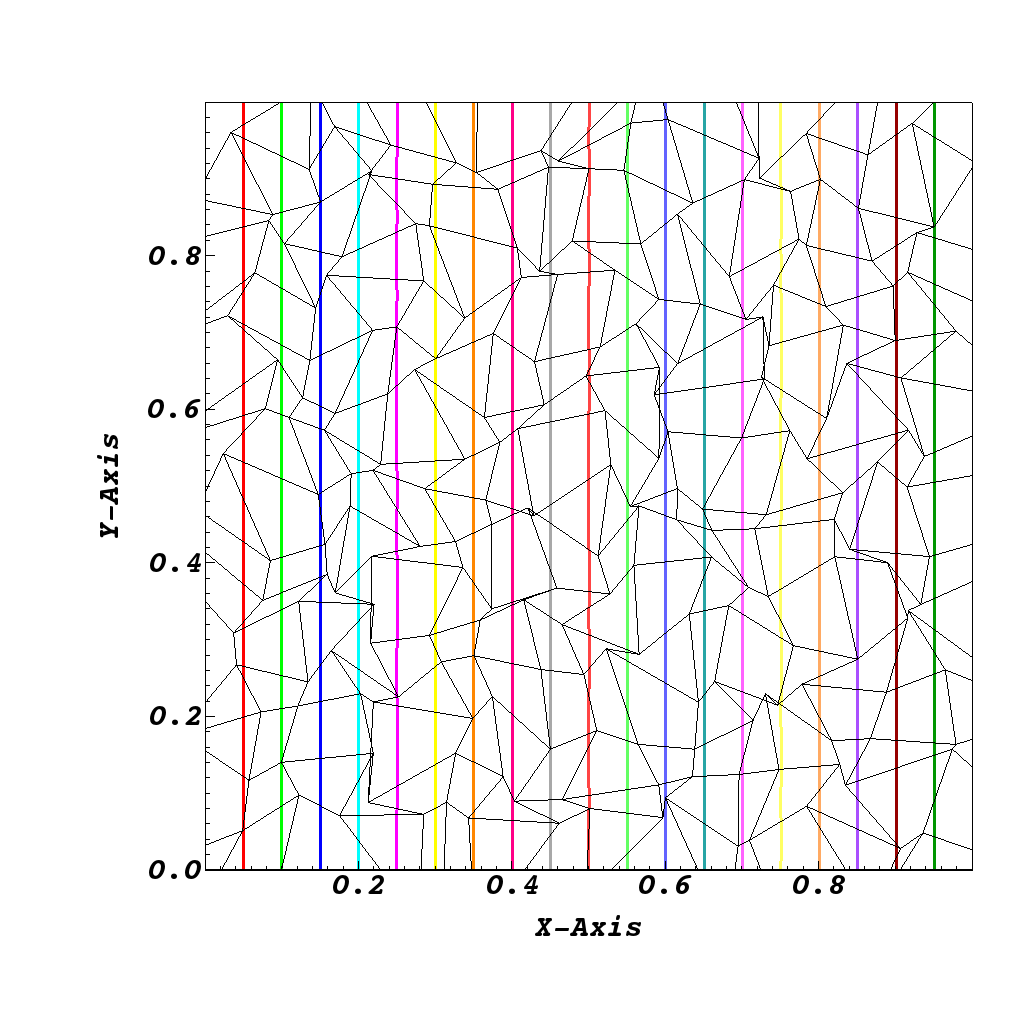
\includegraphics[scale=0.15]{../pwld_diffusion/results/linear/quads/rand/rand_quad_linear_L1_n16_a0_66}
\label{fig:linear_rand_quad}
}
\subfigure[Z-mesh]{
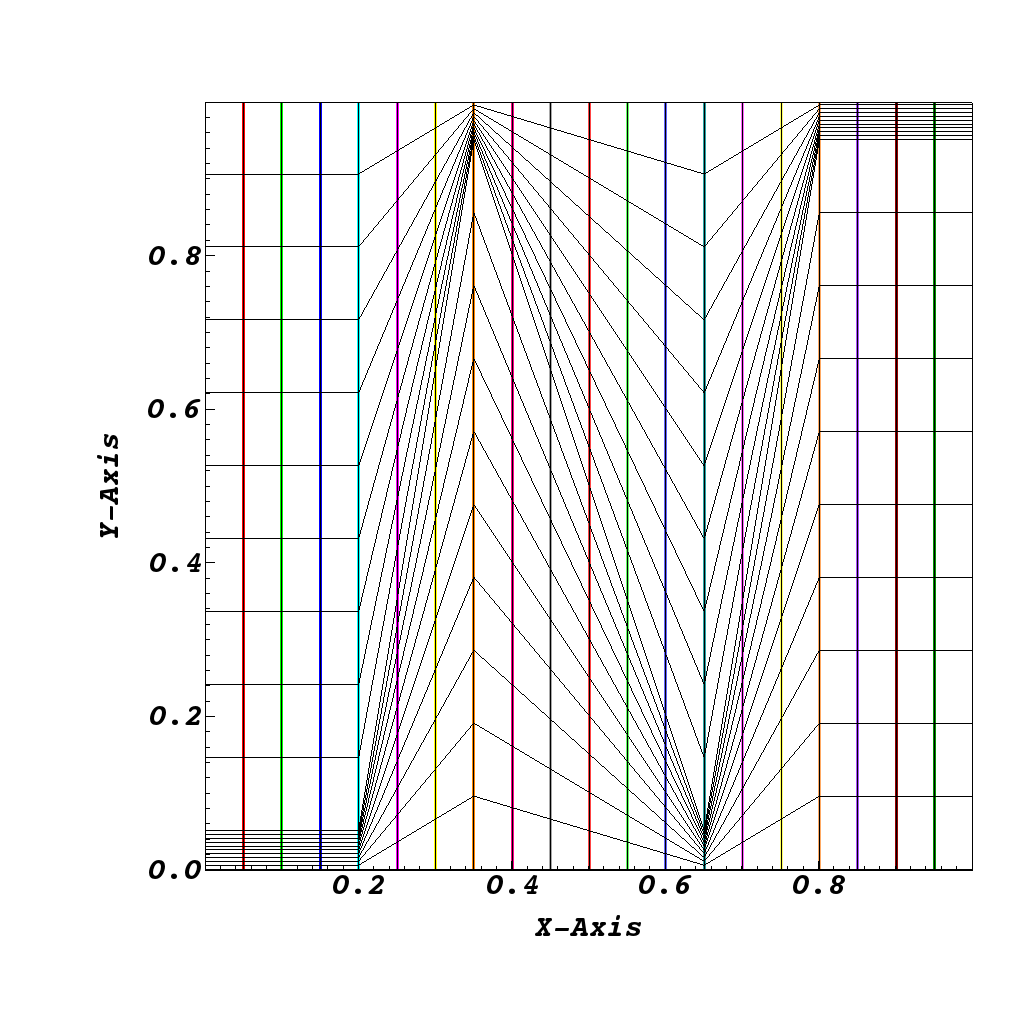
\includegraphics[scale=0.15]{../pwld_diffusion/results/linear/quads/z-mesh/zzzz_quad_linear_L1_n20_a0_05}
\label{fig:linear_z_quad}
}
\subfigure[Shestakov $a=0.15$]{
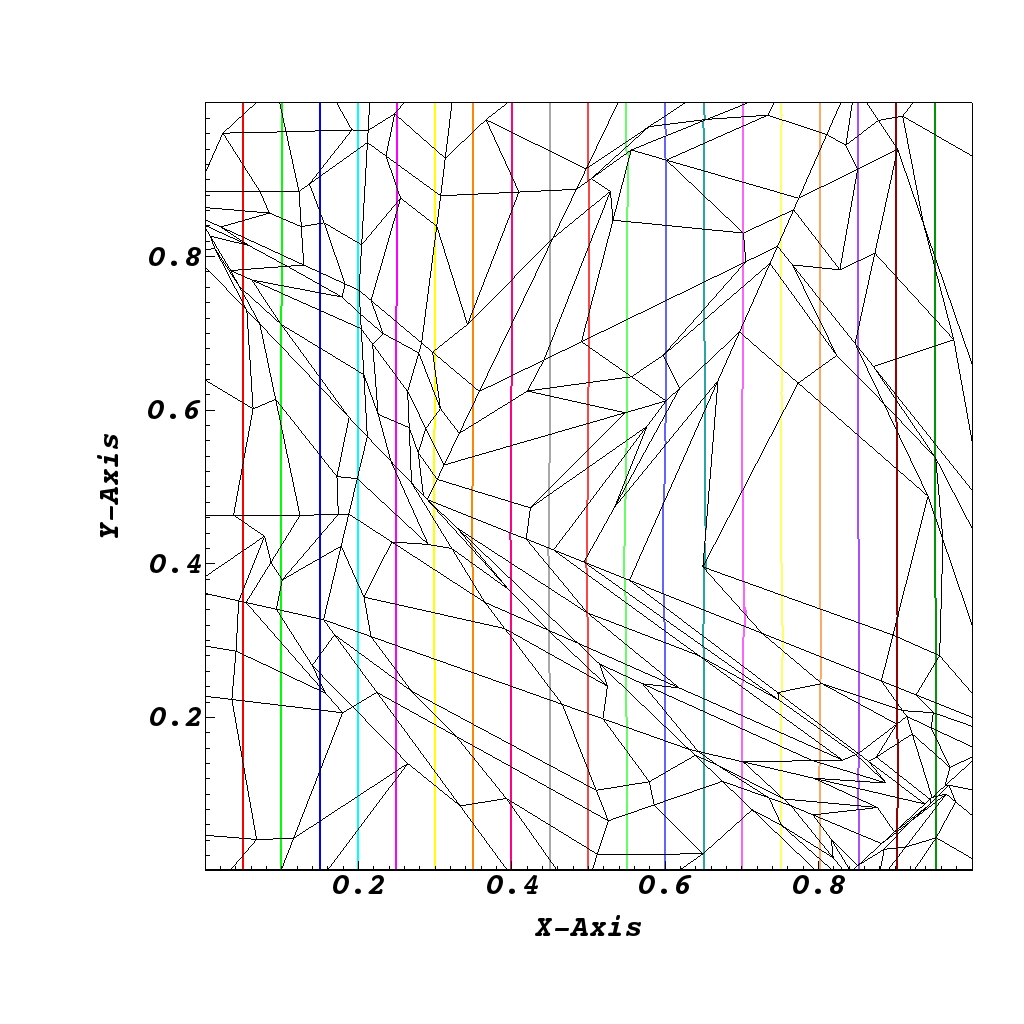
\includegraphics[scale=0.15]{../pwld_diffusion/results/linear/quads/shes/shes_quad_linear_L1_nc4_a0_15}
\label{fig:linear_shes_quad}
}
\subfigure[Shaskov $3\times 3$ mesh]{
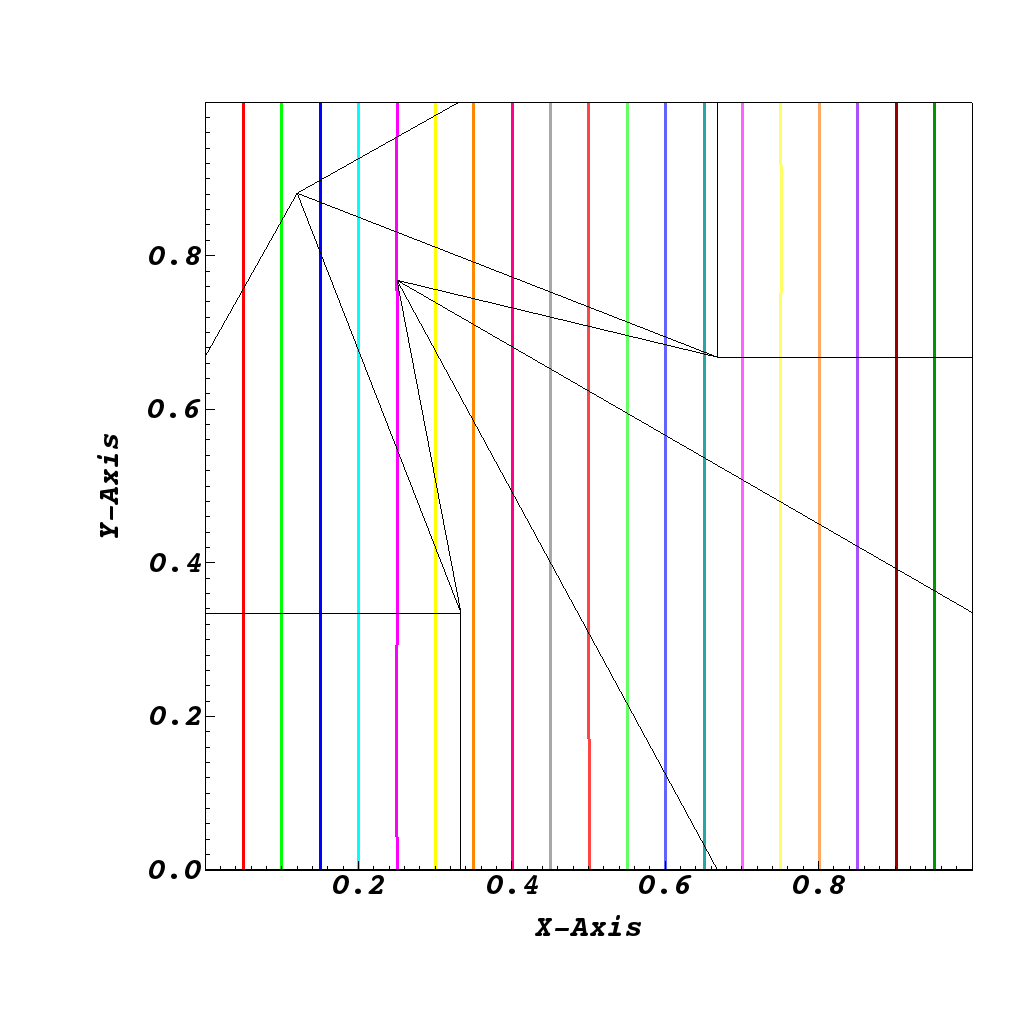
\includegraphics[scale=0.15]{../pwld_diffusion/results/linear/quads/misha}
\label{fig:linear_misha}
}
\caption{Linear solution, 16x16 quads/shes,20x20Z,3x3misha}
\label{fig:linear_quad}
\end{figure}


\begin{table}[htbp]
	\centering
		\begin{tabular}{|l||c|}
		\hline
		Grid      & \# of convex cells / total \# of cells \\ \hline\hline
		Random    & 54 / 256 \\ \hline
		Z-mesh    &  0 / 400 \\ \hline
		Shestakov & 22 / 256 \\ \hline
		Shaskov   &  4 /   9 \\ \hline		
		\end{tabular}
	\caption{Fraction of Concave Cells in Quadrilaterals Grids shown in \fig{fig:linear_quad}}
	\label{tab:FractionOfConcaveCellsInQuadrilateralsGridsShownInFigFig}
\end{table}

rand_poly_linear_L1_n15_a0_95

\end{document}

In this Section, we compare the solution of the problem on an uniform mesh
with the one on Z-mesh \cite{Stone2003}. We also show that the
discretization used can easily handle unstructured polygonal grid. Finally, we
conclude this section with an example of AMR mesh.
\subsection{Z-mesh}
The Z-mesh is defined as in \fig{fig_z_mesh} where $\alpha$ is a parameter
$\in [0,0.5]$. 
\begin{figure}[H]
  \centering
  \includegraphics[width=5cm]{z_mesh}
  \caption{Z-mesh ((x) is the number of divisions and Y is the distance in cm)}
  \label{fig_z_mesh}
\end{figure}    
We compare the solution of the diffusion equation using the Z-mesh
\fig{z_mesh_sol} with $\alpha=0.2$ with the one obtained using an uniform \fig{u_mesh_sol}. 
The domain is 1cm by 1cm and is discretized using 20 by 20 cells. All the 
boundary conditions are vacuum. The medium is homogeneous $\Sigma_a = 0.5 cm^{-1}$ 
and $D=2$. There is a uniform source of intensity 1.                  
\begin{figure}[H]
  \centering
  \includegraphics[width=5cm]{z_mesh_sol}
  \caption{Scalar flux on the z-mesh}
  \label{z_mesh_sol}
\end{figure}
\begin{figure}[H]
  \centering
  \includegraphics[width=5cm]{pwld_uniform_sol}
  \caption{Scalar flux on the uniform mesh}
  \label{u_mesh_sol}
\end{figure}

\subsection{Randomized polygonal grid}

\subsection{AMR}



%%%%%%%%%%%%%%%%%%%%%%%%%%%%%%%%%%%%%%%%%%%%%%%%%%%%%%%%%%%%%%%%%%%%%%%%%%%%%%%%%%%%%%%%%%%%%%%%%%%%
\subsection{Example 1} \label{sec:ex1}
%%%%%%%%%%%%%%%%%%%%%%%%%%%%%%%%%%%%%%%%%%%%%%%%%%%%%%%%%%%%%%%%%%%%%%%%%%%%%%%%%%%%%%%%%%%%%%%%%%%%


%%%%%%%%%%%%%%%%%%%%%%%%%%%%%%%%%%%%%%%%%%%%%%%%%%%%%%%%%%%%%%%%%%%%%%%%%%%%%%%%%%%%%%%%%%%%%%%%%%%%
%%%%%%%%%%%%%%%%%%%%%%%%%%%%%%%%%%%%%%%%%%%%%%%%%%%%%%%%%%%%%%%%%%%%%%%%%%%%%%%%%%%%%%%%%%%%%%%%%%%%
%%%%%%%%%%%%%%%%%%%%%%%%%%%%%%%%%%%%%%%%%%%%%%%%%%%%%%%%%%%%%%%%%%%%%%%%%%%%%%%%%%%%%%%%%%%%%%%%%%%%



%%%%%%%%%%%%%%%%%%%%%%%%%%%%%%%%%%%%%%%%%%%%%%%%%%%%%%%%%%%%%%%%%%%%%%%%%%%%%%%%%%%%%%%%%%%%%%%%%%%%
%%%%%%%%%%%%%%%%%%%%%%%%%%%%%%%%%%%%%%%%%%%%%%%%%%%%%%%%%%%%%%%%%%%%%%%%%%%%%%%%%%%%%%%%%%%%%%%%%%%%
%%%%%%%%%%%%%%%%%%%%%%%%%%%%%%%%%%%%%%%%%%%%%%%%%%%%%%%%%%%%%%%%%%%%%%%%%%%%%%%%%%%%%%%%%%%%%%%%%%%%
\pagebreak

\begin{figure}[h]
\begin{center}
\includegraphics[scale=1.]{two-mesh.eps}
\end{center}
\caption{Schematics of the two-mesh AMR approach.}
\label{fig:2-mesh-schematics}
\end{figure}

%%%%%%%%%%%%%%%%%%%%%%%%%%%%%%%%%%%%%%%%%%%%%%%%%%%%%%%%%%%%%%%%%%%%%%%%%%%%%%%%%%%%%%%%%%%%%%%%%%%%
\pagebreak

\begin{figure}[h]
\begin{center}
\includegraphics[scale=0.4]{ref-rules2.eps}
\end{center}
\caption{Refinement rule: the original triangle is bisected into 4 smaller triangles; 
local numbering rules are defined; a tree structure is employed to obtain the refinement level depth.}
\label{fig:triangle-ref-rule}
\end{figure}

%%%%%%%%%%%%%%%%%%%%%%%%%%%%%%%%%%%%%%%%%%%%%%%%%%%%%%%%%%%%%%%%%%%%%%%%%%%%%%%%%%%%%%%%%%%%%%%%%%%%
\pagebreak

\begin{figure}[!hbtp]
\centering
\subfigure[0-level refinement difference]{
\includegraphics[scale=0.45]{edge-coupling-0}
\label{fig:sub_edge0}
}
\subfigure[1-level refinement difference]{
\includegraphics[scale=0.45]{edge-coupling-1}
\label{fig:sub_edge1}
}
\subfigure[1-level refinement difference]{
\includegraphics[scale=0.45]{edge-coupling-1b}
\label{fig:sub_edge1b}
}
\caption{Cases of edge coupling.}
\label{fig:edge_coupling_fig}
\end{figure}


%%%%%%%%%%%%%%%%%%%%%%%%%%%%%%%%%%%%%%%%%%%%%%%%%%%%%%%%%%%%%%%%%%%%%%%%%%%%%%%%%%%%%%%%%%%%%%%%%%%%

\pagebreak

\begin{figure}[h]
\begin{minipage}[b]{1.\linewidth}
%
\begin{center}
\subfigure[Two-mesh AMR]
{
\includegraphics[width=3.5cm]{mesh-TB-est-2mesh-c14-p-1.ps}
\includegraphics[width=3.5cm]{mesh-TB-est-2mesh-c14-p-2.ps}
\includegraphics[width=3.75cm]{mesh-TB-est-2mesh-c14-p-3.ps}
\includegraphics[width=4.35cm]{mesh-TB-est-2mesh-c14-p-4.ps} 
}
\end{center}
\end{minipage}
%
\begin{minipage}[b]{1.\linewidth}
\begin{center}
\subfigure[Jump-based AMR ]
{
\includegraphics[scale=0.17]{mesh-TB-jump-c14-p1.ps}
\includegraphics[scale=0.17]{mesh-TB-jump-c14-p2.ps}
\includegraphics[scale=0.17]{mesh-TB-jump-c14-p3.ps}
\includegraphics[scale=0.17]{mesh-TB-jump-c14-p4.ps}
}
\end{center}
\end{minipage}
\caption{Example 3: Adapted meshes. From left to right, $p=1,\,2,\,3,\,4$}
\label{fig:ex3-meshes}
\end{figure}


%%%%%%%%%%%%%%%%%%%%%%%%%%%%%%%%%%%%%%%%%%%%%%%%%%%%%%%%%%%%%%%%%%%%%%%%%%%%%%%%%%%%%%%%%%%%%%%%%%%%
%%%%%%%%%%%%%%%%%%%%%%%%%%%%%%%%%%%%%%%%%%%%%%%%%%%%%%%%%%%%%%%%%%%%%%%%%%%%%%%%%%%%%%%%%%%%%%%%%%%%
%%%%%%%%%%%%%%%%%%%%%%%%%%%%%%%%%%%%%%%%%%%%%%%%%%%%%%%%%%%%%%%%%%%%%%%%%%%%%%%%%%%%%%%%%%%%%%%%%%%%
%%%%%%%%%%%%%%%%%%%%%%%%%%%%%%%%%%%%%%%%%%%%%%%%%%%%%%%%%%%%%%%%%%%%%%%%%%%%%%%%%%%%%%%%%%%%%%%%%%%%
%\include{bibli.bib}
%\bibliographystyle{unsrt}
%\bibliography{bibli}

\pagebreak


\begin{thebibliography}{100}


\end{thebibliography}



%%%%%%%%%%%%%%%%%%%%%%%%%%%%%%%%%%%%%%%%%%%%%%%%%%%%%%%%%%%%%%%%%%%%%%%%%%%%%%%%%%%%%%%%%%%%%%%%%%%%
%%%%%%%%%%%%%%%%%%%%%%%%%%%%%%%%%%%%%%%%%%%%%%%%%%%%%%%%%%%%%%%%%%%%%%%%%%%%%%%%%%%%%%%%%%%%%%%%%%%%
\end{document}
%%%%%%%%%%%%%%%%%%%%%%%%%%%%%%%%%%%%%%%%%%%%%%%%%%%%%%%%%%%%%%%%%%%%%%%%%%%%%%%%%%%%%%%%%%%%%%%%%%%%
%%%%%%%%%%%%%%%%%%%%%%%%%%%%%%%%%%%%%%%%%%%%%%%%%%%%%%%%%%%%%%%%%%%%%%%%%%%%%%%%%%%%%%%%%%%%%%%%%%%%
